%\documentclass{Physics_H_Notes}
%\begin{document}
    \chapter[热力学]{\itr{Thermodynamics}{热力学}}
    \begin{solution}[\\In state-of-the-art vacuum systems, pressures as low as $10^{-9}\rm{Pa}$ are being attained. 
        Calculate the number of molecules in a $1.00\rm{m^{3}}$ vessel at this pressure if the temperature is 27°C]
        由理想气体方程$pV=Nk_{_B}T$得:
        \begin{equation*}
            N = \frac{pV}{k_{_B}T} = \frac{10^{-9}\times 1.00}{1.38\times 10^{-23}\times (27+273)} = 2.4 \times 10^{11}
        \end{equation*}
        很简单的题目,一是强调热力学温度单位应统一使用开尔文;二是想说明热力学的题目套公式记得从已知条件出发,
        有人可能会考虑压强的微观表达公式,但这里并没有给出方均根速率,还需要结合麦克斯韦分布,这就显得繁琐了。
    \end{solution}
    \begin{solution}[\\The root-mean-square 
        speed of molecules in air (mostly $\rm{N_2}$) is comparable to 
        the speed of sound in air (or in an ideal gas).\\
        (a) Using the equation of state of an ideal gas, calculate the bulk 
        modulus (at temperature $T$), which is defined as:
        \begin{equation*}
            B = \frac{volume \ stress}{volume \ strain} = -\frac{\Delta F/A}{\Delta V/V} = -\frac{\Delta P}{\Delta V/V}
        \end{equation*}
        (b) Recall that the speed of sound in a fluid $v=\sqrt{B/\rho}$ depends on
        the elastic and inertial properties of the fluid, where $B$ is the bulk
        modulus and $\rho$ is the density of air. Express the speed of sound 
        waves in terms of molecular mass $m$, temperature $T$, as well as 
        the Boltzmann's constant $k_{_B}$.\\
        (c) In fact, the speed of sound has an additional factor of $\sqrt{\gamma}$ ,
        where $\gamma$ is the adiabatic index ($\gamma = 7/5 = 1.400$ for diatomic molecules 
        at room temperature). Compute the result in (b) at room temperature (The molar
        mass of air is $29 \rm{g/mol}$). ]
        读懂题目照着意思写就行。

        (a)根据$pV=nRT$,在温度确定时有$p=\dfrac{nRT}{V}$,即:
        \begin{equation*}
            \Delta p = -\frac{nRT}{V^{2}}\Delta V
        \end{equation*}
        于是代入定义即有:
        \begin{equation*}
            B = -\frac{\Delta P}{\Delta V/V} = \frac{nRT}{V}
        \end{equation*}
        \\
        (b)直接代入即可:
        \begin{equation*}
            v=\sqrt{\frac{B}{\rho}}=\sqrt{\frac{\frac{nRT}{V}}{\frac{nM}{V}}} = \sqrt{\frac{RT}{M}}=\sqrt{\frac{k_{_B}T}{m}}
        \end{equation*}
        \\
        (c)代入数据,注意室温一般取$298\rm{K}$,以及把摩尔质量的单位转化为kg:
        \begin{equation*}
            v=\sqrt{\frac{RT}{M}} =\sqrt{\frac{8.314\times 298}{29\times 10^{-3}}}\rm{m/s} = 342\rm{m/s}
        \end{equation*}
        这一结果与声速常用值$340\rm{m/s}$十分相近。
    \end{solution}
    \begin{solution}[\\The van der Waals equation of state is as follows:
        \begin{equation*}
            (p+\frac{a}{V^{2}})(V-b)=nRT
        \end{equation*}
        (a) Calculate the isothermal compressibility of the van der Waals gas in terms of $(V,T)$ and
        determine the high-temperature limit. How does this result compare to that for an ideal gas?\\
        Hint: The isothermal compressibility $\kappa_T$ is defined through $\kappa_{T}=-\dfrac{1}{V}\left(\dfrac{\partial V}{\partial p}\right)_{T}$\\
        (b) The van der Waals equation possesses a so-called critical point, where
        \begin{equation*}
            \left(\frac{\partial p}{\partial V}\right)_{T} = \left(\frac{\partial^{2} p}{\partial V^{2}}\right)_{T} = 0
        \end{equation*}
        Determine the critical pressure $p_c$, the critical volume $V_c$ and the critical temperature $T_c$. What
        is the behavior of $\kappa_T$ at the critical point?\\
        (c) Use the expressions for $V_c$, $p_c$, and $T_c$ in the van der Waals equation of state and show that it
        assumes a simple form independent of $a$ and $b$ when $T$,$V$, and $p$ are measured in terms of $T_c$,
        $V_c$, $p_c$, $i.e.$, when expressing the van der Waals equation in terms of $T/T_c$ , $V/V_c$ , $p/p_c$]
        本质仍然是一道阅读理解,理解后难度只在计算。

        (a)利用隐函数求导法则两边求导:
        \begin{equation*}
                (V-b)(1-\frac{2a}{V^{3}}\frac{\partial V}{\partial p}) + (p+\frac{a}{V^{2}})\frac{\partial V}{\partial p} = 0 
        \end{equation*}
        整理有:
        \begin{equation*}
            \frac{\partial V}{\partial p} = \frac{-V+b}{\frac{2ab}{V^{3}}-\frac{a}{V^{2}}+p}
        \end{equation*}
        故
        \begin{equation*}
            \kappa_T(p,V) = -\frac{1}{V}\frac{\partial V}{\partial p} = \frac{1-\frac{b}{V}}{\frac{2ab}{V^{3}}-\frac{a}{V^{2}}+p}
        \end{equation*}
        观察范德华状态方程,发现我们可以分离$p$:
        \begin{equation*}
            p = \frac{nRT}{V-b}-\frac{a}{V^{2}}
        \end{equation*}
        代入$\kappa_T$的表达式中,并整理得到:
        \begin{equation*}
            \kappa_T(V,T) = \frac{V^{2}(V-b)^{2}}{nRTV^{3}-2a(V-b)^{2}}
        \end{equation*}
        然后看高温极限,当$T\rightarrow +\infty$时,同样有$V\rightarrow +\infty$。为计算方便我们取$\kappa_{T}(p,V)$,令$V\rightarrow +\infty$:
        \begin{equation*}
            \lim_{T\rightarrow +\infty}\kappa_T = \lim_{V \rightarrow +\infty}\frac{1-\frac{b}{V}}{\frac{2ab}{V^{3}}-\frac{a}{V^{2}}+p}=\frac{1}{p}
        \end{equation*}
        对理想气体$V = \frac{nRT}{p}$,其$\kappa_T$如下:
        \begin{equation*}
            \kappa_T = -\frac{1}{V}\frac{\partial V}{\partial p} = \frac{nRT}{pV^{2}} = \frac{1}{p}
        \end{equation*}
        可以看到范德华气体$\kappa_T$的高温极限与理想气体一致。
        \\
        
        (b)由范德华状态方程分离$p$:
        \begin{equation*}
            p = \frac{nRT}{V-b}-\frac{a}{V^{2}}
        \end{equation*}
        对$V$偏导:
        \begin{equation*}
            \left(\frac{\partial p}{\partial V}\right)_{T} = -\frac{nRT}{(V-b)^{2}} + \frac{2a}{V^{3}} = 0
        \end{equation*}
        继续对$V$偏导:
        \begin{equation*}
            \left(\frac{\partial^{2} p}{\partial V^{2}}\right)_{T} = \frac{2nRT}{(V-b)^{3}} - \frac{6a}{V^{4}} = 0
        \end{equation*}
        整理消去$nRT$即可求出$V_c$:
        \begin{equation*}
            \begin{aligned}
                \frac{2a(V-b)^{2}}{V^{3}} &= nRT = \frac{3a(V-b)^{3}}{V^{4}}\\
                &V_c = 3b
            \end{aligned}
        \end{equation*}
        回代得到$T_c$:
        \begin{equation*}
            T_c = \frac{3a(V_{c}-b)^{3}}{nRV_{c}^{4}} = \frac{8a}{27nRb}
        \end{equation*}
        回代到$p$的表达式中得到$p_c$:
        \begin{equation*}
            p_c = \frac{nRT_c}{V_{c}-b}-\frac{a}{V_{c}^{2}} = \frac{a}{27b^{2}}
        \end{equation*}
        回代到$\kappa_T$的表达式中发现分母有
        \begin{equation*}
            \frac{2ab}{V_{c}^{3}}-\frac{a}{V_{c}^{2}}+p_{c} = 0
        \end{equation*}
        且分子不为0,故在临界点有$\kappa_T\rightarrow +\infty$。
        \\

        (c)其实就是用临界参数来表示$a$、$b$与$R$,这里先用量纲看一下怎么表示好,
        即用$T/T_c$,$V/V_c$,$p/p_c$代替范德华方程中的$T$,$V$,$p$,
        同时用无量纲量$a_{_0}$,$b_{_0}$,$R_{_0}$代替$a$,$b$,$R$:
        \begin{equation*}
            \begin{aligned}
                &(\frac{p}{p_c}+\frac{a_{_0}}{\left(\frac{V}{V_c}\right)^{2}})(\frac{V}{V_c}-b_{_0})=nR_{_0}\frac{T}{T_c}\\
                &(p+\frac{a_{_0}p_{c}V_{c}^2}{V^2})(V-b_{_0}V_c) = n(\frac{R_{_0}p_{c}V_{c}}{T_{c}})T
            \end{aligned}
        \end{equation*}        
        比较一下原来的形式,我们有:
        \begin{equation*}
            \begin{cases}
                a = a_{_0}p_{c}V_{c}^2\\
                b = b_{_0}V_c\\
                R = \dfrac{R_{_0}p_{c}V_{c}}{T_{c}}
            \end{cases}
        \end{equation*}
        下面只需要把临界参数的表达式代入解出三个常数即可,过程略。
        令$T_R = T/T_c$,$V_R = V/V_c$,$p_{_R} = p/p_c$,最后的形式为:
        \begin{equation*}
            (p_{_R}+\frac{3}{V_R^{2}})(V_R-\frac{1}{3})=\frac{8}{3}T_R
        \end{equation*}
    \end{solution}
    \begin{solution}[\\An ideal diatomic gas, in a cylinder with a movable piston, undergoes the rectangular cyclic process shown
        . Assume that the temperature is always such
        that rotational degrees of freedom are active, but vibrational modes are “frozen out.” Also assume that the only
        type of work done on the gas is quasistatic compression-expansion work. \\
        (a) For each of the four steps A through D, compute the work done on the gas, the heat added to
        the gas, and the change in the internal energy of the gas.
        Express all answers in terms of P1, P2, V1, and V2. \\
        (b) Compute the net work done on the gas, the net
        heat added to the gas, and the net change in the internal
        energy of the gas during the entire cycle. Are the results
        as you expected? Explain briefly.]
        \begin{center}
           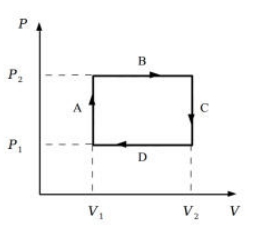
\includegraphics[height=5cm,width=5cm]{Chapter7_pV1.png}
        \end{center}

        基本的$p-V$图计算,注意认清每个过程。根据题意忽略振动对于内能的贡献,所有功均为体积功。
        双原子气体必然为线性分子,则有$i = 5$。

        (a) A为等容过程:
        \begin{equation*}
            \begin{aligned}
                &W_A = 0\\
                &Q_A = \frac{5}{2}R\Delta T = \frac{5}{2}(p_{2}-p_{1})V_1\\
                &\Delta U_A = Q_A = \frac{5}{2}(p_{2}-p_{1})V_1
            \end{aligned}
        \end{equation*}
        B为等压过程:
        \begin{equation*}
            \begin{aligned}
                &W_B = p_2(V_2 - V_1)\\
                &Q_B = \frac{7}{2}R\Delta T = \frac{7}{2}p_{2}(V_2 - V_1)\\
                &\Delta U_B = Q_B - W_B = \frac{5}{2}p_{2}(V_2 - V_1)
            \end{aligned}
        \end{equation*}
        C为等容过程:
        \begin{equation*}
            \begin{aligned}
                &W_C = 0\\
                &Q_C = \frac{5}{2}R\Delta T = \frac{5}{2}(p_{1}-p_{2})V_2\\
                &\Delta U_C = Q_C = \frac{5}{2}(p_{1}-p_{2})V_2
            \end{aligned}
        \end{equation*}
        D为等压过程:
        \begin{equation*}
            \begin{aligned}
                &W_D = p_1(V_1 - V_2)\\
                &Q_D = \frac{7}{2}R\Delta T = \frac{7}{2}p_{1}(V_1 - V_2)\\
                &\Delta U_D = Q_D - W_D = \frac{5}{2}p_{1}(V_1 - V_2)
            \end{aligned}
        \end{equation*}
        (b) 净功为:
        \begin{equation*}
            W = W_B + W_D = (p_2 - p_1)(V_2 - V_1)
        \end{equation*}
        数值上等于循环对于的闭合曲线在$p-V$图中围成的面积(注意一定要是$p-V$图)

        净热量为:
        \begin{equation*}
            Q = Q_A + Q_B + Q_C + Q_D = (p_2 - p_1)(V_2 - V_1)
        \end{equation*}
        净热量等于净功。

        净内能变化量为:
        \begin{equation*}
            \Delta U = \Delta U_A + \Delta U_B + \Delta U_C + \Delta U_D = 0 
        \end{equation*}
        内能为状态函数,由于始态与终态相同,故净内能变化量一定为0。

        对总过程有$\Delta U = Q - W$成立。
    \end{solution}
    \begin{solution}[\\For a van der Waals gas, its equation of state implies a phase transition between
        liquid and gas below a critical temperature $T_c$: In the $P-V$ phase
        diagram, the isothermal line for a given temperature $T_{_0} < T_{c}$ is not monotonically
        decreasing with respect toV, but a constant function of $V$ in some region (see the
        figure). This region corresponds to a phase transition from liquid to gas state (with a
        volume change from $V_{L}^{mol}$ to $V_{G}^{mol}$), and the mole latent heat is $L$ for the transition.
        Suppose we use 1 mole of this van der Waals gas/liquid mixture as the medium for
        a Carnot cycle operating between the high temperature $T_{_0}$ and the low temperature
        $T_{_0}-\Delta T$ — which are connected by two adiabatic processes $D\rightarrow A$ and $B\rightarrow C$.
        The pressure in the flat region changes from $P_{_0}$ to $P_{_0}-\Delta P$ when the temperature
        changes from $T_{_0}$ to $T_{_0}-\Delta T$.\\
        (a) Specify the heat transfer and work done in each process of $A\rightarrow B$, $B\rightarrow C$,
        $C\rightarrow D$, and $D\rightarrow A$ in such a Carnot cycle. Here, we assume that the volume
        change in $B\rightarrow C$ and $D\rightarrow A$ is negligible.\\
        (b) Calculate the total work done to the environment for this Carnot cycle and express
        its efficiency $\epsilon$ from $\epsilon = W/Q_H$. where $W$ and $Q_H$ is the total work output in
        the cycle and the heat input at the high temperature, respectively\\
        (c) For a Carnot engine with efficiency $\epsilon = 1-\frac{T_C}{T_H}$, verify the Clapeyron equation:
        \begin{equation*}
            \frac{\dif{P}}{\dif{T}}=\frac{L}{T(V_{G}^{mol}-V_{L}^{mol})}
        \end{equation*}    
        for the liquid/gas mixture.]
        \begin{center}
           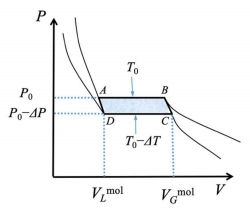
\includegraphics[height=5cm,width=6cm]{Chapter7_pV2.png}
        \end{center}
        (a) 注意对理想气体成立的结论对范德华气体不再成立。

        $A\rightarrow B$是等压相变过程,由于假设,体积变化量视为$V_{G}^{mol}-V_{L}^{mol}$:
        \begin{equation*}
            \begin{aligned}
                &W_1 = p\Delta V = p_{_0}(V_{G}^{mol}-V_{L}^{mol})\\
                &Q_1 = L
            \end{aligned}
        \end{equation*}

        $B\rightarrow C$与$D\rightarrow A$为绝热过程,故$Q_2 = Q_4 = 0$。

        至于范德华气体绝热过程下功的计算,我怀疑这是否是题目的本意,这里姑且给出计算方法。

        首先我们利用范德华方程得到$p$的表达式:
        \begin{equation*}
            p = \frac{RT}{V - b} - \frac{a}{V^2}
        \end{equation*}
        内能对$T$,$V$两个变量全微分:
        \begin{equation*}
            \dif U = \left(\frac{\partial U}{\partial T}\right)_{V} \dif T + \left(\frac{\partial U}{\partial V}\right)_{T} \dif V
        \end{equation*}
        不难注意到全微分的前一项$\left(\dfrac{\partial U}{\partial T}\right)_{V} = C_{V}$,至于后一项,我们需要先得到普适的能态方程。

        熵对$T$,$V$两个变量全微分:
        \begin{equation*}
            \dif S = \left(\frac{\partial S}{\partial T}\right)_{V} \dif T + \left(\frac{\partial S}{\partial V}\right)_{T} \dif V
        \end{equation*}
        代入热力学基本方程中:
        \begin{equation*}
            \dif U = T\dif S - p \dif V 
            = T\left(\frac{\partial S}{\partial T}\right)_{V} \dif T + \left[T\left(\frac{\partial S}{\partial V}\right)_{T} - p\right] \dif V
        \end{equation*}
        定义亥姆霍兹自由能$A=U-TS$,关于其热力学基本方程为            
        \begin{equation*}
            \dif{A} = \dif U - \dif (TS) = \dif U - T \dif S - S \dif T = -S\dif{T} - p\dif{V}
        \end{equation*}
        利用二元函数全微分的必要条件,即偏导次序可交换,有下面的关系,称为麦克斯韦关系(之一):
        \begin{equation*}
            \left(\frac{\partial S}{\partial V}\right)_{T} 
            =\left[\frac{\partial}{\partial V}\left(\frac{\partial A}{\partial T}\right)_V \right]_T 
            =\left[\frac{\partial}{\partial T}\left(\frac{\partial A}{\partial V}\right)_T \right]_V 
            =\left(\frac{\partial p}{\partial T}\right)_{V}
        \end{equation*}
        从而得到下面的式子,事实上被称为能态方程:
        \begin{equation*}
            \left(\frac{\partial U}{\partial V}\right)_{T} = T\left(\frac{\partial p}{\partial T}\right)_{V} - p
        \end{equation*}
        将范德华气体的状态方程代入,有:
        \begin{equation*}
            \left(\frac{\partial U}{\partial V}\right)_{T} = \frac{RT}{V-b} - p = \frac{a}{V^{2}}
        \end{equation*}
        这样我们就得到了范德华气体内能的微分形式:
        \begin{equation*}
            \dif U = C_{V}\dif T + \frac{a}{V^{2}}\dif V
        \end{equation*}
        积分有(可以证明,事实上范德华气体的$C_{V} = C_{V}(T)$,与体积无关):
        \begin{equation*}
            \Delta U = \int_{T_1}^{T_2}C_{V}\dif T + \frac{a}{V_1} - \frac{a}{V_2} 
        \end{equation*}
        从而根据热力学第一定律$\Delta U = -W$:
        \begin{equation*}
            \begin{aligned}
                & W_2 = \int_{T_{_0}-\Delta T}^{T_{_0}}C_{V}\dif T - \frac{a}{V_{B}} + \frac{a}{V_{G}^{mol}}  \\
                & W_4 = -\int_{T_{_0}-\Delta T}^{T_{_0}}C_{V}\dif T + \frac{a}{V_{A}} - \frac{a}{V_{L}^{mol}} 
            \end{aligned}
        \end{equation*}
        根据题目后面来看,它应该是认为$W_2 = -W_4$。

        $C\rightarrow D$ 是等压相变过程,由于相变热$L$与温度相关,且根据题目的意思也没法用克拉伯龙方程,这里用热力学第一定律计算:
        \begin{equation*}
            \begin{aligned}
                &W_3 = p\Delta V = -(p_{_0} - \Delta p)(V_{G}^{mol}-V_{L}^{mol})\\
                &Q_3 = W - Q_1 = \Delta p(V_{G}^{mol}-V_{L}^{mol}) - L
            \end{aligned}
        \end{equation*}
        
        (b) 利用(a)中的结果代入即可:
        \begin{equation*}
            \epsilon = \frac{W}{Q_H} = \frac{\Delta P(V_{G}^{mol}-V_{L}^{mol})}{L}
        \end{equation*}

        (c) 在这里$T_H = T_{_0}$,$T_C =T_{_0} - \Delta T$,代入有:
        \begin{equation*}
            \epsilon = \frac{\Delta P(V_{G}^{mol}-V_{L}^{mol})}{L} = \frac{\Delta T}{T_{_0}}
        \end{equation*}
        对近平衡可逆过程,用$\dif T$与$\dif p$代替$\Delta T$与$\Delta p$,并移项,即有:
        \begin{equation*}
            \frac{\dif{P}}{\dif{T}}=\frac{L}{T(V_{G}^{mol}-V_{L}^{mol})}
        \end{equation*}
    \end{solution}
    \begin{solution}[\\ Consider the Carnot cycle operating with a hot and cold heat baths whose temperatures are $T_h$ and
        $T_c$ ($T_h > T_c$), respectively. Working substance means the gas in the engine, and we consider a gas in
        general for the working substance.\\
        (a) Suppose the amount of heat exchange during the isothermal process with the hot (cold) heat bath is
        $Q_h$ ($Q_c$), and determine the entropy change $\Delta S_h$ and $\Delta S_c$ of the working substance in the respective
        process. Then, specify $\Delta S_h$ and $\Delta S_c$ are positive or negative. Here, take the positive sign of $Q_h$
        and $Q_c$ for the heat input from the heat bath to the working substance.\\
        (b) Now we use an ideal gas as the working substance and consider a free expansion process. Suppose the
        initial temperature of the gas is $T_i$ and the volume of the gas increases from $V_i$ to $V_f$. Determine the
        heat input $Q_{fe}$ and the entropy change $\Delta S_{fe}$ of the working substance through the free expansion
        process.\\
        (c) By replacing a quasi-static isothermal expansion process in the Carnot cycle by a free expansion
        process, it seems that it is possible to construct a cycle with a single heat bath. Does this fact
        violate the second law of thermodynamics? Answer by yes or no, then explain your answer using
        the case of the Carnot cycle.]
        (a) 等温过程,高温时系统吸热,低温时系统放热,代入熵的定义中:
        \begin{equation*}
            \begin{aligned}
                &\Delta S_h = \frac{Q_h}{T_h}\\
                &\Delta S_c = -\frac{Q_c}{T_c}
            \end{aligned}
        \end{equation*}

        (b) 自由膨胀,有外界真空$W = 0$与绝热$Q_{fe} = 0$。

        熵变则利用熵是状态函数与自由膨胀始态与终态温度相等的特性,用等温过程连接始态与终态,熵变为:
        \begin{equation*}
            \Delta S_{fe} = nR\ln{\frac{V_f}{V_i}}
        \end{equation*}

        (c) 否。因为自由膨胀并不是一个可逆过程,压缩时会导致外界环境发生变化,符合热力学第二定律。
    \end{solution}
%\end{document}